\documentclass[11pt, letterpaper]{article}
% --- FONT CONFIGURATION ---
\usepackage[T1]{fontenc}
\usepackage{lmodern}
\usepackage{float}
% --- FORMATTING PACKAGES ---
\usepackage[margin=1in]{geometry}
\linespread{1.2}
\setlength{\parskip}{0.5\baselineskip}
\setlength{\parindent}{0pt}
\usepackage{amsmath,amssymb}
\usepackage{newtxtext,newtxmath}
\usepackage{graphicx}
\usepackage{xcolor}
\definecolor{docnotelinkcolor}{rgb}{0,0,0}
\frenchspacing
\usepackage{booktabs}
\usepackage{threeparttable}
\usepackage{placeins}
\usepackage{caption}
\usepackage{bbm}
\setcounter{secnumdepth}{4}
\usepackage[numbers,sort&compress]{natbib}
\usepackage{url}
\usepackage{hyperref}
\hypersetup{colorlinks=true,linkcolor=black,citecolor=black,urlcolor=black}
\captionsetup{font=scriptsize, labelfont=bf}
\newcommand{\parencite}[1]{\cite{#1}}
\newcommand{\textcite}[1]{\cite{#1}}

\title{\textbf{Resources, Not Rank: Fiscal Capacity Drives the Diffusion of Occupationally Relevant Skills into U.S.\ Higher-Education Curricula}}
\author{}
\date{}

\begin{document}
\maketitle

\begin{abstract}
Public disinvestment in higher education is known to affect access, costs and completion. Whether it also changes what students are taught is less clear. Here we study the diffusion of occupationally relevant skills into U.S.\ higher-education curricula by linking the Course-Skill Atlas of college syllabi (2000--2017) to Carnegie classifications and federal finance, staffing and enrollment records. We measure curricular specialization with a Revealed-Comparative-Advantage index across 1,500 institutions and 62 fields of study, identifying 41.9 million skill-adoption and 42.1 million skill-abandonment opportunities. Descriptively, elite research universities appear to update curricula faster: Carnegie R1 institutions adopt frontier occupational skills more rapidly ($b=0.331$, $p<0.001$) and abandon them more slowly ($b=-0.192$, $p<0.001$). But this prestige gradient does not survive the strongest available status-based tests, which exploit the timing of Carnegie reclassification through event-study and generalized synthetic-control designs. By contrast, fiscal exposure to the 2008 recession does predict curricular change. Institutions that depended more heavily on state appropriations before the crisis subsequently adopted fewer frontier skills and abandoned fewer existing ones ($p<0.01$ for both), with effects emerging after several years and strengthening through 2017. The same temporal pattern appears in instructional staffing: state-dependent institutions experienced a significant decline in instructional staff headcount ($b=-0.038$, $p<0.0001$), while instructional expenditure per student was largely preserved. These findings suggest that curricular modernization is constrained less by institutional rank itself than by the organizational capacity that fiscal resources sustain.
\end{abstract}

\clearpage
\section*{Introduction}

Public disinvestment in higher education is usually discussed as a story about cost and access: can students still afford to enroll, and will they finish. That framing leaves out a more basic question--what happens to the content of their education once resources tighten. Higher-education curricula are not static content; they are organizational artifacts that change--or fail to change--as institutions decide which occupationally relevant skills to teach \parencite{autorskill2003, javadiansabet2024}. A long sociological tradition holds that such organizational change diffuses hierarchically: elite organizations adopt innovations first, and the rest of the field follows, emulating practices that carry the endorsement of high-status actors \parencite{podolny1993, phillipszuckerman2001, strangsoule1998, dimaggiopowell1983}. Applied to higher education, this account predicts that elite research universities should be the first to update their curricula toward emerging occupational skill demands, with regional and mass-access institutions catching up--if at all--only after a lag. This prediction is intuitive, widely assumed in policy discussions of curricular ``innovation,'' and, as we show below, strongly supported by a naive correlational analysis of the very data we use to test it. The stakes extend well beyond higher-education policy narrowly construed: if the skills millions of students learn each year are governed by an institution's fiscal circumstances rather than by which institutions are best positioned to sense labor-market change, then curricular change is not simply a story about organizations imitating prestige--it is a channel through which macroeconomic shocks and the state's fiscal choices reshape the content of mass human-capital formation, and, by extension, the workforce readiness and life chances of the students who pass through the least prestigious, most state-dependent parts of the system.

It is also, we argue, not the whole causal story.

Status-cascade accounts of diffusion are notoriously difficult to test causally, because institutional status is not randomly assigned: whatever unobserved characteristics make an institution elite--research intensity, applicant quality, endowment, faculty ambition--are also plausible independent drivers of curricular dynamism, and status itself is measured with categories (Carnegie classifications) that a body external to any single institution assigns on a schedule that institutions do not control. Recent work on faculty hiring networks shows that U.S.\ academic status hierarchies are steep, self-reinforcing, and consequential for who is hired where \parencite{clauset2015}; whether the same hierarchy structures \emph{what is taught}, and not merely \emph{who is hired}, is a distinct empirical question that--to our knowledge--has not been subjected to causal identification at scale. One possibility, which we take seriously throughout, is that status and resources are not rival explanations but stages in a single causal chain: status may operate largely \emph{through} its effect on an institution's ability to acquire fiscal resources, rather than exerting an independent effect on curricular capacity once resources are held fixed \parencite{clauset2015}.

We address it using the Course-Skill Atlas \parencite{javadiansabet2024}, a national longitudinal dataset that maps millions of U.S.\ course syllabi (2000--2017) onto the O*NET occupational skill architecture, linked to Carnegie institutional classifications and to federal (IPEDS/NCES) records of institutional finance, staffing, and enrollment. We first replicate the standard correlational finding: institutional prestige strongly and significantly predicts both faster adoption and slower abandonment of frontier occupational skills. We then ask whether that association survives the strongest status-based variation available in these data: the timing of Carnegie reclassification. Using both a Sun-and-Abraham event-study estimator \parencite{sunabraham2021, goodmanbacon2021} and a generalized synthetic-control design \parencite{xu2017}, we find little evidence that crossing into a higher status tier directly accelerates curricular skill diffusion. Additional exploratory designs--regression discontinuity, peer-network IV, and institutional mergers--are useful diagnostics but are not treated as primary evidence because they either fail at the first stage, rely on a weak proxy network, or capture a broader organizational shock rather than status itself.

We then ask what \emph{does} drive it. Exploiting the 2008 recession as an aggregate shock with heterogeneous exposure across institutions--and using real, institution-level state-appropriation data from IPEDS Finance rather than a coarse public/private proxy--we find a robust, temporally coherent, and mechanistically traceable causal effect: institutions with greater pre-recession state-appropriation dependence (the share of operating revenue an institution draws from state government, our term for this construct throughout) experienced significantly slower curricular adoption and abandonment after 2009, an effect that emerges only after several years and grows monotonically through the end of our panel. We trace this pattern to a parallel, similarly lagged decline in instructional staffing, while nominal instructional spending, once normalized by enrollment, is essentially unaffected--consistent with institutions protecting per-student instructional budgets while shedding the staff capacity needed to revise and extend curricula. We emphasize at the outset that this resource-dependence finding rests principally on one well-identified natural experiment (the 2008 recession), supplemented by a second, weaker test that corroborates it only partially (see Results); we do not claim symmetric multi-design support for the resource channel of the kind we sought, and did not find, for the status channel.

Our contribution is threefold. First, we assemble and correct a large novel panel linking curricular skill content to institutional prestige and finance at a scale (hundreds of millions of institution$\times$field$\times$skill$\times$year observations) not previously available for this question. Second, we show that a canonical status-cascade finding, replicated here with standard associational methods, is not supported by the most defensible status-based tests available in the data. Third, we identify and trace the mechanism of an alternative, resource-dependence account \parencite{pfeffersalancik1978} of curricular change, with implications for how state disinvestment in public higher education reverberates through the content of what is taught, not merely through access and affordability.

\subsection*{Theoretical framework}

Two accounts compete to explain why some institutions update their curricula toward occupationally relevant skills faster than others.

The \emph{status-cascade} account holds that high-status organizations act as focal points that lower-status organizations emulate, and that status itself confers the legitimacy, resources, and market position needed to innovate first \parencite{podolny1993, phillipszuckerman2001, strangsoule1998}. Empirically, this account predicts a monotonic association between institutional prestige and the pace of curricular adoption--precisely the pattern we replicate in our associational baseline--and is consistent with evidence that academic status hierarchies are steep and self-reproducing in other domains, such as faculty hiring \parencite{clauset2015}.

The \emph{resource-dependence} account instead holds that organizational change requires discretionary organizational capacity--administrative staff to revise curricula, faculty lines to teach new content, budget to absorb the transition costs of curricular reform--and that this capacity is a function of an organization's fiscal position vis-\`a-vis its environment, not of its status per se \parencite{pfeffersalancik1978}. For U.S.\ public higher education, state appropriations are a first-order determinant of that fiscal position, and cuts to state appropriations are known to depress a wide range of institutional outcomes \parencite{demingwalters2017}. On this account, prestige and curricular dynamism are correlated not because status causes dynamism, but because both are downstream of resources: well-resourced institutions tend to be both prestigious and fiscally comfortable, so a purely correlational design cannot separate the two channels.

These two accounts are not necessarily mutually exclusive alternatives. A plausible mediation story--consistent with, though not directly tested by, the demonstration that academic status hierarchies are steep and self-reinforcing in faculty hiring \parencite{clauset2015}--holds that status operates on curricular change \emph{indirectly}, by helping institutions acquire the fiscal and administrative resources that in turn enable curricular revision (status $\rightarrow$ resource acquisition $\rightarrow$ curricular capacity), rather than status and resources being cleanly severable causes that compete for the same variance. Our design strategy--holding status fixed via exogenous-variation designs, and separately isolating exogenous variation in fiscal resources--is well suited to asking whether status has an effect \emph{net of, or independent from,} resource variation, but it does not by itself adjudicate the full mediation chain. We therefore frame our central claim throughout as: no independent status channel is detectable once resource variation is isolated, rather than the stronger and less defensible claim that status is irrelevant to curricular change in general.

Distinguishing between these accounts requires isolating variation in status, or in resources, that is plausibly independent of the confounders that generate the observed correlation--precisely the ``reflection problem'' that has long bedeviled empirical work on status and peer effects \parencite{manski1993}. We therefore first use Carnegie reclassification to test whether institutional rank itself changes curricular dynamics, and then use the 2008 recession to isolate variation in fiscal exposure directly.

\section*{Results}

\subsection*{Data and the associational baseline}

We measure curricular skill specialization using a Revealed Comparative Advantage (RCA) framework analogous to that used in economic-complexity research \parencite{balassa1965, hidalgohausmann2009}. For each institution$\times$field-of-study cell (unit of analysis: 1,500 institutions $\times$ 62 fields of study, 2000--2017) and each of 2,412 Detailed Work Activities (DWAs) drawn from O*NET, we compute
$$
\mathrm{RCA}_{c,p,t} = \frac{X_{c,p,t}/\sum_{p'} X_{c,p',t}}{\sum_{c'} X_{c',p,t}/\sum_{c',p'} X_{c',p',t}},
$$
where $X_{c,p,t}$ is the total syllabus-level relevance score of skill $p$ in cell $c$ at year $t$, and where $c$, $p$, $t$ index institution$\times$field cells, skills, and years respectively (in Methods, we index the same three dimensions as $i$, $j$, $t$--institution, field, and year--where $i\equiv c$ and $j\equiv p$; we use $(c,p,t)$ here to match the economic-complexity RCA literature and $(i,j,t)$ in Methods to match the panel-econometric hazard-model literature). A cell is coded as specialized in (``having'') a skill when $\mathrm{RCA} \geq 1$; adoption and abandonment are defined as $0\rightarrow1$ and $1\rightarrow0$ transitions in this indicator. This criterion, unlike a naive presence threshold, is selective by construction (mean specialization rate 45.5\%, versus $\sim$99\% under a raw score-presence rule; see Methods), and yields 41.9 million adoption and 42.1 million abandonment opportunities across the top 100 status-asymmetric (``frontier'') skills.

\begin{table}[H]
\centering
\caption{Associational baseline: discrete-time hazard model of frontier-skill adoption and abandonment as a function of exposure and institutional prestige (binary R1 status, Model~1--2; ordinal prestige tier and discipline-level prestige concentration, in the source code's ``gradient'' specification). Model includes year and field-of-study fixed effects only (no institution fixed effect); standard errors are IID (not clustered), as reported in the table footnote.}
\label{tab:main1}

\begingroup
\centering
\begin{tabular}{lcccc}
   \tabularnewline \midrule \midrule
   Dependent Variable: & \multicolumn{4}{c}{evento}\\
    & \multicolumn{4}{c}{Adopcion (bin.)} \\ 
    & \multicolumn{4}{c}{Adopcion (grad.)} \\ 
    & \multicolumn{4}{c}{Abandono (bin.)} \\ 
    & \multicolumn{4}{c}{Abandono (grad.)} \\ 
   Model:                     & (1)             & (2)             & (3)             & (4)\\  
   \midrule
   \emph{Variables}\\
   exp\_elite\_z              & 0.2348$^{***}$  & 0.2390$^{***}$  & 0.0754$^{***}$  & 0.0734$^{***}$\\   
                              & (0.0056)        & (0.0056)        & (0.0060)        & (0.0060)\\   
   exp\_base\_z               & -0.3964$^{***}$ & -0.4033$^{***}$ & -0.2556$^{***}$ & -0.2534$^{***}$\\   
                              & (0.0053)        & (0.0053)        & (0.0056)        & (0.0056)\\   
   is\_r1                     & 0.3310$^{***}$  &                 & -0.1925$^{***}$ &   \\   
                              & (0.0020)        &                 & (0.0020)        &   \\   
   prestige\_tier\_num        &                 & 0.1144$^{***}$  &                 & -0.0613$^{***}$\\   
                              &                 & (0.0007)        &                 & (0.0007)\\   
   field\_status\_index\_z    &                 & -0.0420$^{***}$ &                 & -0.0115$^{***}$\\   
                              &                 & (0.0042)        &                 & (0.0041)\\   
   \midrule
   \emph{Fixed-effects}\\
   year                       & Yes             & Yes             & Yes             & Yes\\  
   fos                        & Yes             & Yes             & Yes             & Yes\\  
   \midrule
   \emph{Fit statistics}\\
   Observations               & 6,405,909       & 6,405,909       & 5,487,589       & 5,487,589\\  
   Squared Correlation        & 0.04698         & 0.04702         & 0.07908         & 0.07876\\  
   Pseudo R$^2$               & 0.03893         & 0.03894         & 0.06256         & 0.06232\\  
   BIC                        & 7,602,798.8     & 7,602,778.3     & 6,710,225.0     & 6,711,957.2\\  
   \midrule \midrule
   \multicolumn{5}{l}{\emph{IID standard-errors in parentheses}}\\
   \multicolumn{5}{l}{\emph{Signif. Codes: ***: 0.01, **: 0.05, *: 0.1}}\\
\end{tabular}
\par\endgroup



\end{table}

A discrete-time hazard model regressing adoption and abandonment on system-wide exposure to elite and non-elite adopters, institutional Carnegie status, and year and field fixed effects reproduces the canonical status-cascade pattern (Table~\ref{tab:main1}). Carnegie R1 institutions adopt frontier skills significantly faster than other institutions ($b=0.331$, $p<0.001$) and abandon them significantly more slowly ($b=-0.192$, $p<0.001$); an ordinal institutional-prestige gradient and a discipline-level prestige-concentration index reproduce the same pattern ($b=0.114$ and $b=-0.061$ for adoption and abandonment, respectively, both $p<0.001$). In substantive terms, on the logistic scale a coefficient of $b=0.331$ corresponds to an odds ratio of about 1.39--R1 institutions' odds of adopting a given frontier skill in a given year are roughly 39\% higher than non-R1 institutions' odds, holding exposure and fixed effects constant; the abandonment coefficient of $b=-0.192$ corresponds to an odds ratio of about 0.83, an approximately 17\% lower odds of abandonment. Taken at face value, this is precisely what a status-cascade account predicts, and it is the sort of evidence on which the broader literature on prestige-driven diffusion typically rests. The skill set underlying these estimates--the 100 skills with the largest baseline (2000--2001) gap in specialization between R1 and non-R1 institutions--is fixed \emph{before} the 2001--2017 window over which adoption and abandonment are measured, so this asymmetry is not manufactured by the outcome window itself (see Methods).

\subsection*{Descriptive characterization: three skill types, weak raw gradients}

Before turning to causal identification, we pause to characterize descriptively the phenomenon that the causal designs below will interrogate. This section is a secondary, non-causal exercise--it asks whether the raw, unadjusted patterns in the data already look like a clean status gradient, not whether status \emph{causes} curricular change--and readers primarily interested in the paper's causal argument can proceed directly to the next section without loss of continuity; full design-by-design detail supporting the characterization below is in Methods and the Supplementary Materials. We classify each of the 2,070 curricular skills with adequate baseline prevalence into one of three types, following the logic of prior work on occupational skill polarization but adapted to an external, non-circular source: functional domain (Socio-Cognitive vs.\ Sensory-Physical) is assigned from the official O*NET Content Model hierarchy--each Detailed Work Activity's parent Generalized Work Activity branch, where branch 4.A.3 (``Work Output'') is defined by O*NET as physical activities, equipment, and vehicle operation, and the remaining branches (Information Input, Mental Processes, Interacting with Others) are analytical or social in content (671 Sensory-Physical skills; 1,416 Socio-Cognitive). We then split the Socio-Cognitive class at the within-domain median of a nestedness-contribution score computed from our own institution$\times$field specialization matrix (704 General, 703 Specialized; 9 additional Socio-Cognitive skills at extreme baseline prevalence lack a valid nestedness-contribution score and are excluded from this specificity split, though retained in the domain-level Socio-Cognitive count of 1,416), analogous to prior work on skill hierarchies. (An initial attempt classified functional domain using the same co-specialization network method as the occupational-skill literature, applied to our institution$\times$field cells instead of occupations; it failed to recover a coherent cognitive/physical split, instead recovering disciplinary bundling--e.g., ``Give medications or immunizations'' and ``Analyze costs and benefits of proposed designs'' were assigned to the same cluster. We report this failure in Methods because it clarifies why domain classification requires an external criterion in this setting, unlike for occupations.) This negative result is itself substantively informative, and we flag it as such rather than only as a methodological footnote: it suggests that the ``natural,'' data-driven clustering of curricular skills in our setting is organized around disciplinary bundling (which skills a given academic program teaches together), not around the cognitive/physical functional distinction that structures occupational skill polarization. This raises a genuine open question about how much analytical work the a priori O*NET domain split is doing in our descriptive cross-tabulations below, as opposed to a discipline-based typology that we do not pursue further in this paper; we flag this as a limitation of the descriptive (though not the causal) analyses.

Cross-tabulating adoption and abandonment rates by skill type and institutional prestige tier reveals a phenomenon with real but \emph{modest} raw gradients--unlike the sharp, monotonic status gradients found for occupational skill diffusion. Adoption rates by prestige tier (0 = non-doctoral to 3 = R1-elite) are nearly flat for Sensory-Physical skills (31.5\% at tier~0 to 31.7\% at tier~3) and for Specialized Socio-Cognitive skills (29.6\% to 30.5\%), and if anything decline slightly for General Socio-Cognitive skills (33.3\% to 32.0\%). Abandonment rates tell a more differentiated story: Specialized Socio-Cognitive skills are abandoned notably less often at R1 institutions (38.3\% at tier~0 vs.\ 36.9\% at tier~3), while General Socio-Cognitive skills are abandoned \emph{more} often at R1 institutions (36.3\% to 37.5\%)--opposite gradients within the same broad cognitive domain. Cross-tabulating by discipline-level prestige concentration (terciles of the field-status index) shows a similar lack of a single dominant gradient: General Socio-Cognitive adoption peaks in disciplines with \emph{middling} elite concentration (35.8\%, vs.\ 31.5\% and 30.8\% in the low- and high-concentration terciles), not at either extreme. Full cross-tabulations are reported in the Supplementary Materials.

This descriptive weakness is itself informative: the strong, significant coefficients in the pooled associational model (Table~\ref{tab:main1}) are not the surface expression of a uniform, monotonic prestige gradient visible in the raw data across skill types and disciplines. They emerge only once system-wide exposure and fixed effects are added--consistent with a pooled estimate that is more fragile to confounding than it first appears, and motivating a more focused test of whether institutional status itself drives curricular change.

\subsection*{Status-based tests provide little support for a direct prestige effect}

We then asked whether this association reflects a direct effect of status, or selection: institutions on a rising trajectory of research intensity and resources may both attain elite status \emph{and} update curricula for reasons that precede classification. The most defensible status-based variation in our data comes from the timing of Carnegie reclassification. Carnegie categories are revised on a fixed external schedule (2000, 2005, 2010, 2015 within our window), so the moment at which an institution crosses into a higher research tier is less directly chosen by the institution than its status in any given cross-section. We therefore treat Carnegie reclassification as the primary test of the status-cascade account and estimate it in two complementary ways: a Sun-and-Abraham event study and a generalized synthetic-control design (Table~\ref{tab:status}).

\begin{table}[H]
\centering
\scriptsize
\caption{Primary status-based tests of Carnegie reclassification on frontier-skill adoption and abandonment. ATT = average treatment effect on the treated.}
\label{tab:status}
\begin{threeparttable}
\begin{tabular}{lcc}
\toprule
Design & ATT (adoption) & ATT (abandonment) \\
\midrule
Event-study (Sun--Abraham) & $-0.006$ ($p=0.55$) & $-0.005$ ($p=0.71$) \\
Generalized synthetic control & $-0.001$ ($p=0.92$) & $-0.024$ ($p=0.13$) \\
\bottomrule
\end{tabular}
\begin{tablenotes}
\scriptsize
\item The event-study estimate for abandonment has pre-trend concerns; the generalized synthetic-control design is included to target that weakness directly.
\end{tablenotes}
\end{threeparttable}
\end{table}

Restricting to \emph{clean} transitions--promotions or demotions that do not reverse for the remainder of the panel, which rules out boundary institutions that merely oscillate across the cutoff between classification cycles--we identify 140 clean promotions and 103 clean demotions. A Sun-and-Abraham event-study estimator, which avoids the negative-weighting pathologies of naive staggered-timing designs \parencite{goodmanbacon2021, sunabraham2021}, finds no significant average effect of promotion on either adoption ($\mathrm{ATT}=-0.006$, $p=0.55$) or abandonment ($\mathrm{ATT}=-0.005$, $p=0.71$), though the abandonment flow shows scattered pre-treatment differences that complicate interpretation (Fig.~\ref{fig:reclass}, panel~1). A generalized synthetic-control design \parencite{xu2017}, which reweights the donor pool to reproduce each treated institution's pre-treatment trajectory, directly addresses that concern. It also finds no detectable effect on adoption ($\mathrm{ATT}=-0.001$, $p=0.92$) and a suggestive but non-significant reduction in abandonment ($\mathrm{ATT}=-0.024$, $p=0.13$), with cleaner pre-treatment fit (Fig.~\ref{fig:reclass}, panel~2).

\begin{figure}[H]
\centering
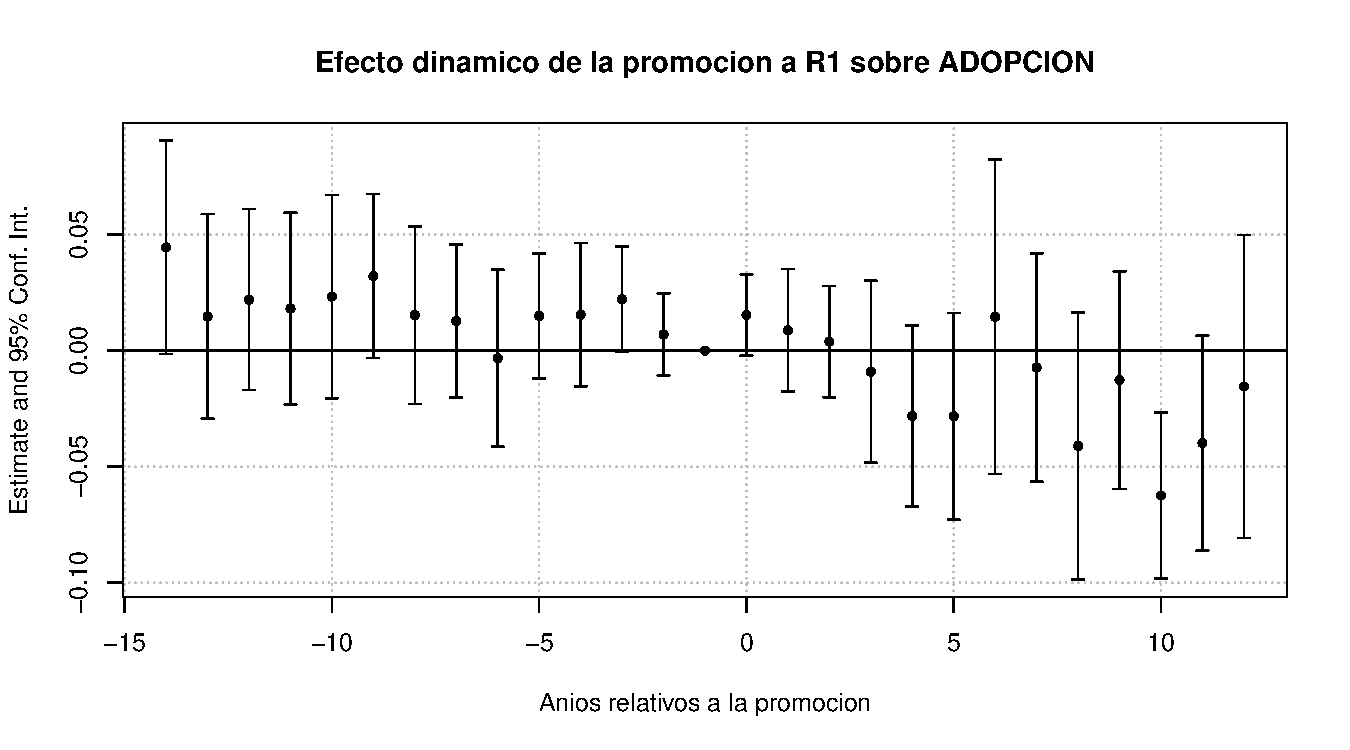
\includegraphics[width=0.48\textwidth,page=1]{figures/event_study_reclasificacion.pdf}
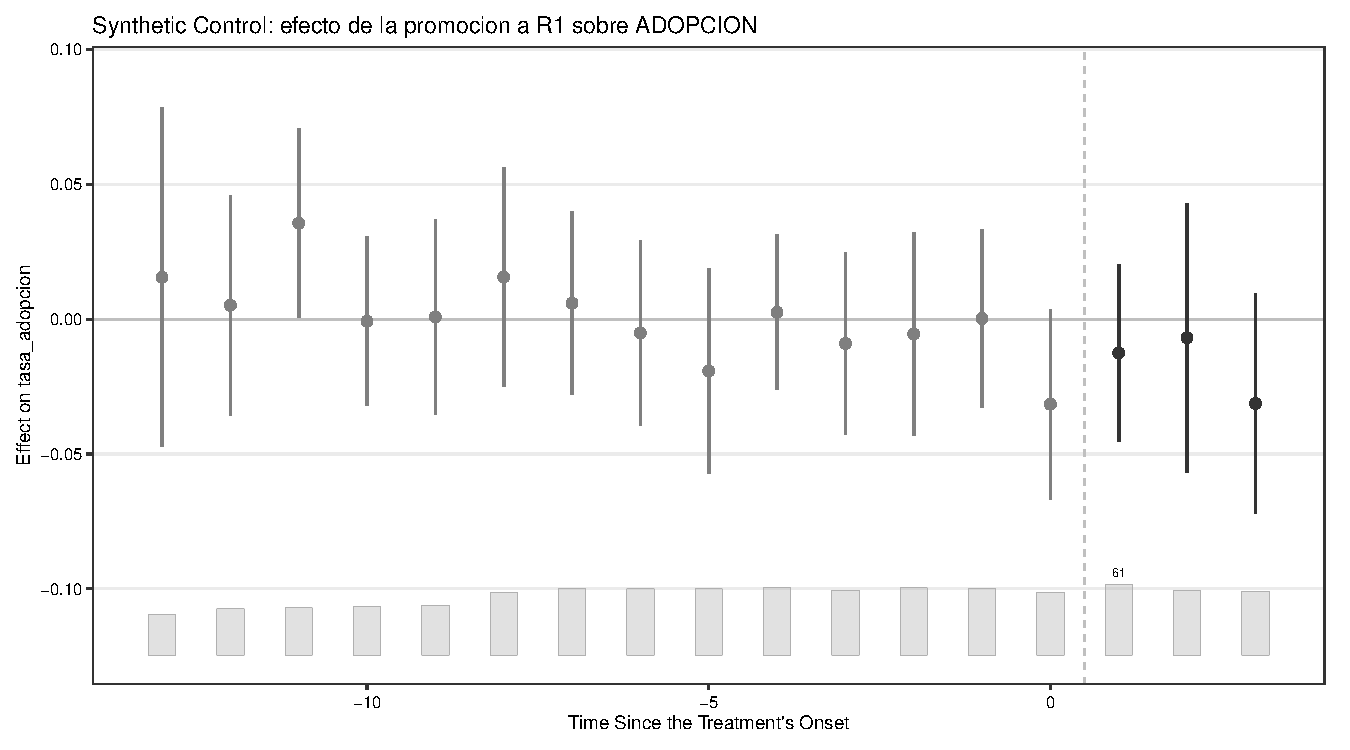
\includegraphics[width=0.48\textwidth,page=1]{figures/synthetic_control_reclasificacion.pdf}
\caption{Dynamic effect of Carnegie reclassification on frontier-skill adoption. Left: Sun--Abraham event-study coefficients by year relative to promotion. Right: generalized synthetic-control estimate of the average treatment effect on the treated, with pre-treatment fit.}
\label{fig:reclass}
\end{figure}

Additional designs were explored but are not used as central evidence. Two regression-discontinuity attempts around the research-intensity threshold fail at the first stage, and therefore are non-informative rather than null results. A peer-network instrumental-variable design is limited by a weak first stage and by the fact that its network is based on structural similarity rather than observed contact. An event study of institutional mergers captures a broader organizational shock, not a clean status shock. These exercises are useful as diagnostics and robustness checks, but the main status-based evidence rests on Carnegie reclassification. Taken together, those primary tests do not support a direct causal prestige effect comparable to the large associational gradient in Table~\ref{tab:main1}.

\subsection*{Fiscal capacity, not status, causally predicts curricular change}

We then turned to a resource-dependence account of the same outcome. The 2008 recession triggered sharp, well-documented cuts to state appropriations for public higher education \parencite{demingwalters2017}, a shock common in timing across institutions but heterogeneous in intensity: institutions differ substantially in how dependent their operating revenue is on state government. We measured this dependence directly from IPEDS Finance records--institution-level state appropriations as a share of total revenue, averaged over 2005--2007 to fix a pre-recession baseline (mean dependence: 29.3\% for public institutions, 0.3\% for private nonprofits, 0.7\% for private for-profits, an institution-type contrast consistent with the well-documented differential exposure of public institutions to state budget cycles). We call this measure \emph{state-appropriation dependence} and use that term consistently throughout the remainder of the paper; we use it as a continuous treatment-intensity variable in a difference-in-differences design with a common event date (2009).

\begin{table}[H]
\centering
\caption{Effect of pre-recession state-appropriation dependence (standardized, 2005--2007 baseline) interacted with a post-2009 indicator on frontier-skill adoption (Model~1), abandonment (Model~2), and log instructional expenditure (Model~3, public institutions only, nominal, not FTE-normalized). Standard errors clustered by institution in parentheses.}
\label{tab:main2}

\begingroup
\centering
\begin{tabular}{lccc}
   \tabularnewline \midrule \midrule
   Dependent Variables: & \multicolumn{2}{c}{evento} & log\_gasto\_instruccion\\
    & \multicolumn{3}{c}{Adopcion} \\ 
    & \multicolumn{3}{c}{Abandono} \\ 
    & \multicolumn{3}{c}{log(Gasto Instruccion)} \\ 
   Model:                                  & (1)             & (2)             & (3)\\  
   \midrule
   \emph{Variables}\\
   baseline\_share\_z                      & 0.1559          &                 &   \\   
                                           & (43,804.3)      &                 &   \\   
   exp\_elite\_z                           & 0.0350$^{***}$  & 0.0042          &   \\   
                                           & (0.0048)        & (0.0047)        &   \\   
   exp\_base\_z                            & -0.0582$^{***}$ & -0.0386$^{***}$ &   \\   
                                           & (0.0045)        & (0.0045)        &   \\   
   post2009 $\times$ baseline\_share\_z    & -0.0069$^{***}$ & -0.0063$^{**}$  & 0.0063\\   
                                           & (0.0024)        & (0.0025)        & (0.0095)\\   
   \midrule
   \emph{Fixed-effects}\\
   unitid                                  & Yes             & Yes             & Yes\\  
   fos                                     & Yes             & Yes             & \\  
   year                                    & Yes             & Yes             & Yes\\  
   \midrule
   \emph{Fit statistics}\\
   Observations                            & 6,387,416       & 5,477,450       & 26,095\\  
   R$^2$                                   & 0.06653         & 0.09100         & 0.96035\\  
   Within R$^2$                            & 0.00283         & 0.00448         & $9.45\times 10^{-5}$\\   
   \midrule \midrule
   \multicolumn{4}{l}{\emph{Clustered (unitid) standard-errors in parentheses}}\\
   \multicolumn{4}{l}{\emph{Signif. Codes: ***: 0.01, **: 0.05, *: 0.1}}\\
\end{tabular}
\par\endgroup



\vspace{-0.5\baselineskip}
{\scriptsize\emph{Note:} the \texttt{baseline\_share\_z} main-effect row in Model~1 (coefficient $0.1559$, SE~$=43{,}804.3$) is not separately identified: this variable is time-invariant at the institution level and is mechanically absorbed by the institution fixed effects included in all three models, so its reported coefficient and standard error are an artifact of estimation and should not be interpreted substantively. Only the \texttt{post2009}~$\times$~\texttt{baseline\_share\_z} interaction, which varies within institution over time, is identified and reported in the main text.\par}
\end{table}

The results are shown in Table~\ref{tab:main2} and Fig.~\ref{fig:recession}. Institutions with greater pre-recession state-appropriation dependence experienced significantly slower adoption of frontier occupational skills after 2009 ($b=-0.0069$ per standard deviation of pre-recession dependence, $p=0.008$) and significantly slower abandonment ($b=-0.0063$, $p=0.020$). Because treatment timing is common across institutions (unlike the staggered Carnegie reclassification), this design is not subject to the negative-weighting critique that motivates the Sun--Abraham estimator \parencite{goodmanbacon2021}, and a standard two-way fixed-effects specification is appropriate.

\begin{figure}[H]
\centering
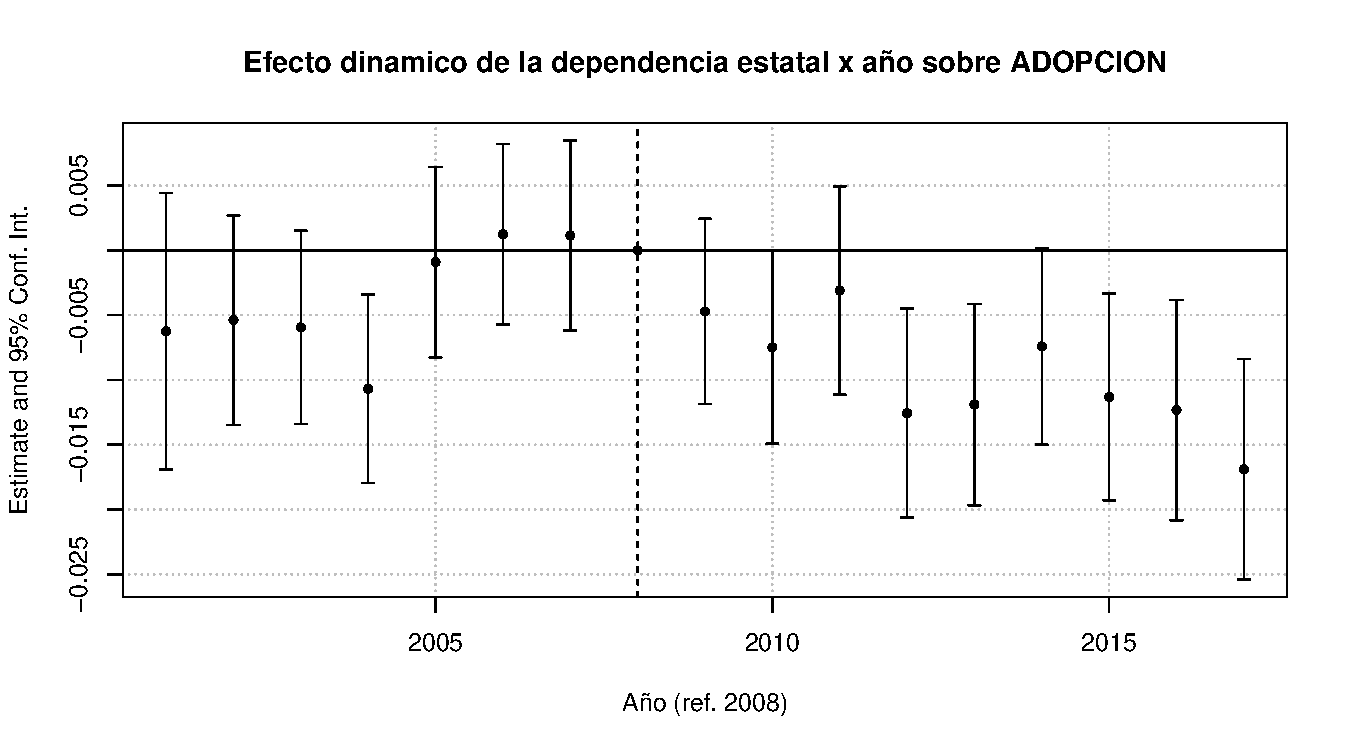
\includegraphics[width=0.48\textwidth,page=1]{figures/recesion_financiamiento_real.pdf}
\includegraphics[width=0.48\textwidth,page=2]{figures/recesion_financiamiento_real.pdf}
\caption{Dynamic effect of pre-recession state-appropriation dependence on frontier-skill adoption (left) and abandonment (right), by year relative to 2008. Coefficients are the interaction of calendar year with standardized pre-recession state-appropriation dependence.}
\label{fig:recession}
\end{figure}

The dynamic (year-by-year) specification is more informative than this average effect, and is also the basis on which we assess the parallel-trends assumption underlying this design rather than simply asserting it. Pre-treatment coefficients (2001--2007) are almost uniformly non-significant and show no visible trend in Fig.~\ref{fig:recession}, which is the evidence supporting parallel trends prior to treatment; we treat this as supportive rather than dispositive, since pre-trend tests have limited power to detect small trend violations. The post-treatment effect on adoption is \emph{not} significant in 2009--2011 and then becomes significant and grows monotonically from 2012 through 2017 (from $b=-0.011$ to $b=-0.014$). We interpret this lag as substantively expected, rather than as a symptom of a delayed or spurious trend violation, because of the specific institutional mechanics of state higher-education budgeting: state appropriations to public institutions are typically set through multi-year budget and biennial appropriation cycles, and institutions facing a state revenue shortfall in 2008--2009 commonly drew down reserves, deferred cuts, or received one-time federal stabilization funds (e.g., ARRA) before state general-fund appropriations were durably reduced in subsequent budget cycles; a multi-year gap between the onset of a fiscal shock and its full transmission to campus staffing and curricular capacity is therefore the pattern this specific institutional process would predict, not an anomaly requiring an alternative explanation. This lagged, cumulative signature is difficult to reconcile with a spurious or mechanically generated association, and is precisely the pattern one would expect if multi-year fiscal retrenchment gradually eroded institutions' capacity to revise curricula.

\subsection*{Mechanism: staffing capacity, not instructional spending}

\begin{table}[H]
\centering
\caption{Effect of pre-recession state-appropriation dependence interacted with a post-2009 indicator on log total instructional staff headcount, 2002--2017. Standard errors clustered by institution in parentheses.}
\label{tab:main3}

\begingroup
\centering
\begin{tabular}{lc}
   \tabularnewline \midrule \midrule
   Dependent Variable:                     & log\_staff\\   
   Model:                                  & (1)\\  
   \midrule
   \emph{Variables}\\
   post2009 $\times$ baseline\_share\_z    & -0.0384$^{***}$\\   
                                           & (0.0092)\\   
   \midrule
   \emph{Fixed-effects}\\
   unitid                                  & Yes\\  
   year                                    & Yes\\  
   \midrule
   \emph{Fit statistics}\\
   Observations                            & 83,952\\  
   R$^2$                                   & 0.90197\\  
   Within R$^2$                            & 0.00107\\  
   \midrule \midrule
   \multicolumn{2}{l}{\emph{Clustered (unitid) standard-errors in parentheses}}\\
   \multicolumn{2}{l}{\emph{Signif. Codes: ***: 0.01, **: 0.05, *: 0.1}}\\
\end{tabular}
\par\endgroup



\end{table}

To identify the channel through which fiscal dependence constrains curricular change, we linked our panel to IPEDS Human Resources records on instructional staffing (2002--2017, spanning a 2012 survey redesign that we harmonize; see Methods) and to IPEDS Finance records on expenditure by functional category, normalized by IPEDS Fall Enrollment full-time-equivalent (FTE) counts. Total instructional staff headcount fell significantly more, after 2009, in institutions with greater state-appropriation dependence ($b=-0.038$ per standard deviation of state-appropriation dependence, $p<0.0001$; Table~\ref{tab:main3}), with a dynamic pattern (Fig.~\ref{fig:mechanism}) that closely mirrors the curricular outcome itself: no significant effect in 2009--2011, followed by a significant and monotonically growing decline from 2012 through 2017 (from $b=-0.028$ to $b=-0.037$). In substantive terms, on the log-staffing scale a coefficient of $b=-0.038$ corresponds to an approximately 3.7\% reduction in instructional staff headcount per standard deviation of pre-recession state-appropriation dependence by the later years of the panel--a modest-sounding but cumulative and durable erosion of the pool of faculty and instructional staff available to develop and teach new curricular content, concentrated among the institutions most exposed to state budget cuts.

\begin{figure}[H]
\centering
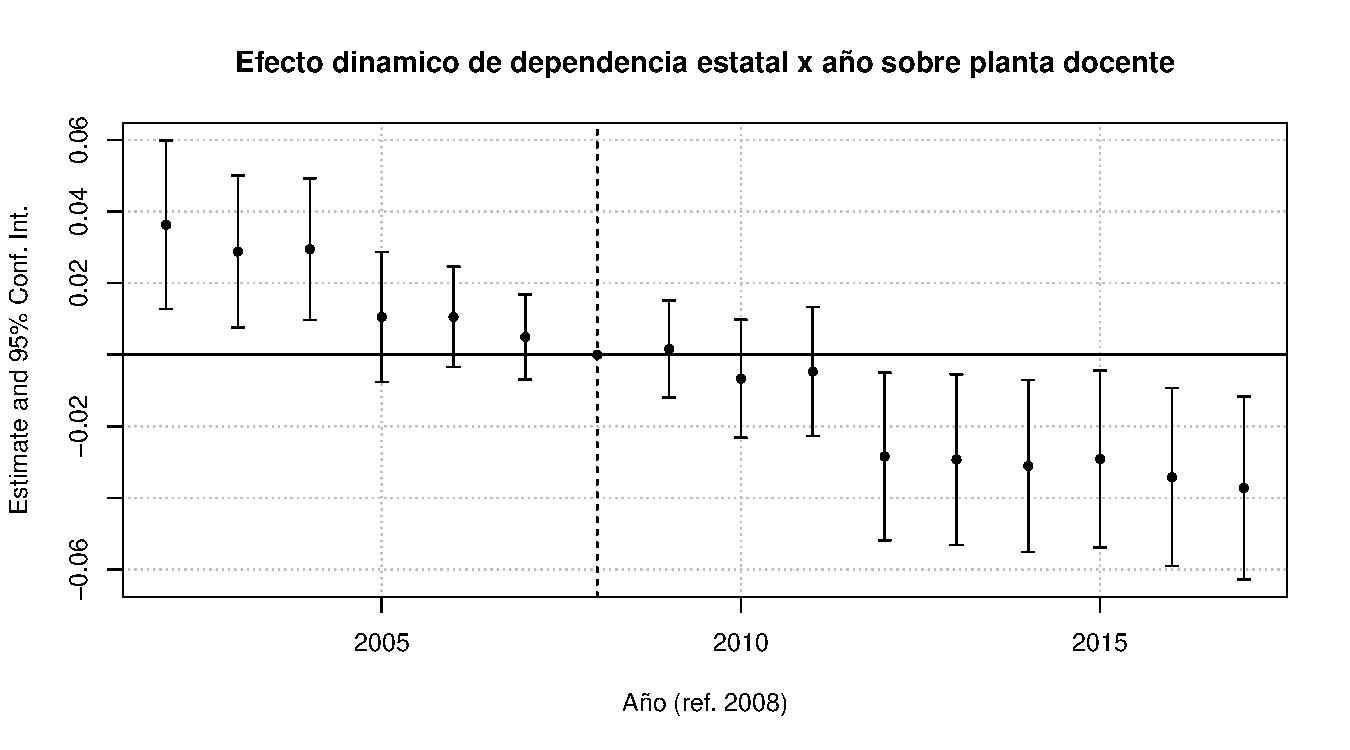
\includegraphics[width=0.7\textwidth,page=1]{figures/mecanismo_planta_docente.pdf}
\caption{Dynamic effect of pre-recession state-appropriation dependence on total instructional staff headcount, by year relative to 2008. The temporal signature closely replicates the curricular outcome in Fig.~\ref{fig:recession}: no effect through 2011, then a significant, monotonically growing decline from 2012 onward.}
\label{fig:mechanism}
\end{figure}

By contrast, nominal instructional expenditure showed no corresponding decline; if anything, several nominal expenditure categories rose relatively faster in more dependent institutions, plausibly reflecting enrollment growth or a shift of the funding burden onto tuition. Once we normalize expenditure by FTE enrollment, the picture clarifies (Table~\ref{tab:main4}): operations-and-maintenance spending per student fell significantly in more dependent institutions ($b=-0.025$, $p=0.019$)--consistent with deferred-maintenance being among the first categories cut in fiscal downturns--while instructional expenditure per student showed no significant change ($b=+0.007$, $p=0.449$), and total expenditure per student rose modestly ($b=+0.022$, $p=0.020$). This last result is worth incorporating explicitly into the mechanism narrative: total per-student expenditure did not fall in more state-dependent institutions after 2009--if anything it rose slightly--even as instructional staff headcount fell. Read together, this pattern is consistent with institutions substituting away from labor-intensive instructional capacity (with its downstream curricular-revision function) while shifting some of the funding burden onto tuition and enrollment growth to keep aggregate and per-student spending levels roughly intact; O\&M spending, in contrast, appears to have been cut directly rather than substituted for. We treat staffing and O\&M spending as two related but analytically distinct channels through which fiscal dependence manifests--both are significant and both point toward real resource constraint--while instructional expenditure per student, the category most proximate to the curricular outcome we study, does not show the same decline, which is why we single out staffing rather than spending as the primary traced mechanism for curricular capacity specifically.

\begin{table}[H]
\centering
\caption{FTE-enrollment-normalized functional expenditure per student, post-2009 $\times$ pre-recession state-appropriation dependence interaction, alongside the staffing coefficient from Table~\ref{tab:main3} for comparison. Standard errors clustered by institution in parentheses; source: \texttt{06k\_mechanism\_expenditure\_per\_fte.R}. Full model output is provided in Supplementary Materials.}
\label{tab:main4}
\begin{threeparttable}
\begin{tabular}{lcc}
\toprule
Outcome (per-FTE, unless noted) & Coefficient & $p$-value \\
\midrule
Instructional staff headcount (log, Table~\ref{tab:main3}) & $-0.038$ & $<0.0001$ \\
Operations \& maintenance expenditure per FTE & $-0.025$ & $0.019$ \\
Instructional expenditure per FTE & $+0.007$ & $0.449$ \\
Total expenditure per FTE & $+0.022$ & $0.020$ \\
\bottomrule
\end{tabular}
\end{threeparttable}
\end{table}

\subsection*{A second, partly independent test of the resource channel}

The recession design rests on a single natural experiment. To gauge whether the resource mechanism is a general property of the data or an artifact of 2008 specifically, we re-estimate its central prediction using an entirely different source of variation: year-over-year growth in each institution's own real state appropriations (2002--2017), interacted with no single event date, so that a cut in \emph{any} year is allowed to predict slower adoption and abandonment the following year. We present this test in the interest of transparency about what it does and does not corroborate, rather than as a second independent design supporting the headline result with equal force. Across the full panel, a one-standard-deviation larger appropriations cut predicts significantly higher abandonment the following year ($b=-0.0046$ on log-growth, $p=0.027$); the corresponding adoption coefficient is small and not significant ($p=0.63$). When the 2008--2011 window is excluded entirely, the abandonment coefficient falls by roughly a third and loses conventional significance ($b=-0.0033$, $p=0.169$). Taken together, this test corroborates the abandonment channel outside the recession window, but not the adoption channel, and even the abandonment corroboration weakens substantially once the recession years themselves are excluded. The honest summary is: this check asks whether the resource effect is confined to the 2008 shock, and the answer is largely yes--most of the identifying power for the resource-dependence account in this paper comes from the 2008 natural experiment specifically, with this second test providing partial, not full, independent replication. A future test exploiting a second large, discrete resource shock--rather than continuous year-to-year variation, which is more exposed to reverse causality and measurement error in short-run appropriations data--would be needed to fully separate a general resource mechanism from a 2008-specific one.

\section*{Discussion}

The standard status-cascade account of organizational diffusion predicts that prestigious institutions should be first to update their offerings toward emerging occupational skill demands, with the rest of the field following at a lag set by relative status. Our associational baseline reproduces this prediction cleanly--it is exactly the pattern a large literature on organizational status and diffusion would lead us to expect \parencite{podolny1993, phillipszuckerman2001, clauset2015}. Yet the strongest status-based tests available here, based on Carnegie reclassification and generalized synthetic controls, do not find that crossing into a higher status tier directly accelerates curricular diffusion. This does not prove that status is irrelevant. Rather, it shows that the large cross-sectional prestige gradient is not, by itself, credible evidence of a direct status-cascade mechanism. The more defensible interpretation is selection: institutions that become prestigious are already on trajectories of resources, staffing and research capacity that also make curricular updating easier.

What does survive causal scrutiny is a resource-dependence account, though we are careful here about the strength of the underlying evidentiary base. Using real, institution-level state-appropriation data rather than a coarse public/private proxy, we show that state-appropriation dependence predicts significantly slower curricular adoption and abandonment following the 2008 recession, with a lagged, monotonically strengthening temporal signature that we are able to trace to a parallel decline in instructional staffing (and, to a lesser extent, in operations-and-maintenance spending) rather than in per-student instructional spending. This central finding rests on one well-identified natural experiment--the 2008 recession--supplemented by a second, year-over-year appropriations-growth test that corroborates the abandonment channel outside the recession window but not the adoption channel, and that weakens substantially once the recession years are excluded; we present this as a single strong causal design plus a partial robustness check, not as convergent evidence from two fully independent natural experiments. This is, to our knowledge, among the first demonstrations that state disinvestment in public higher education has consequences not just for access, cost, and completion--the outcomes on which this literature has traditionally focused \parencite{demingwalters2017}--but for the substantive content of what is taught.

These results speak directly to the comparison that motivated this study: work on academic status hierarchies, most influentially the demonstration that faculty hiring networks are steep and self-reinforcing \parencite{clauset2015}, has established that prestige structures \emph{who} moves through the academic system. Our results are best read not as showing that this hierarchy is irrelevant to curricular content, but that we do not find evidence for an \emph{independent} status channel in the strongest status-based tests we can construct. A plausible reconciliation is that status operates on curricular capacity largely by helping institutions secure the fiscal resources--state appropriations, endowment, tuition-setting power--that in turn enable curricular revision, rather than status exerting a direct effect net of resources. This is a meaningful qualification of status-cascade accounts of organizational diffusion more broadly \parencite{strangsoule1998, dimaggiopowell1983}: status and resources are often treated as complementary or even interchangeable predictors of organizational dynamism, but they should not be interpreted as equivalent mechanisms.

An important alternative interpretation of the fiscal-dependence result, which we cannot fully rule out with the current design, is that our state-appropriation-dependence measure proxies institutional mission or sector as much as it proxies fiscal capacity per se. Community colleges, regional public universities, and other institutions with an explicit vocational or workforce-training mandate tend to be both highly dependent on state appropriations and subject to distinct, non-fiscal channels of curricular pressure--state legislative mandates tied to workforce outcomes, program-approval regimes specific to these sectors, and mission-driven responsiveness to regional labor markets--that could generate a similar post-2008, lagged, growing signature for reasons other than a pure loss of fiscal/staffing capacity. Testing whether the fiscal-dependence effect holds within institutional-type or sector strata (e.g., separately among community colleges, regional publics, and research universities) would be an important robustness check; we have not conducted that stratified analysis in the current version of this paper, and we flag it explicitly as a limitation and a priority for the next round of revision rather than asserting a within-stratum result we have not run. Relatedly, we cannot fully rule out that regional recession severity, differential enrollment or student-composition shocks, or slower-moving secular trends--including 2010s state workforce-curriculum policy mandates that may themselves correlate with state-appropriation dependence--could generate a similar lagged, growing signature; the pre-trend evidence in Fig.~\ref{fig:recession} and the specificity of the staffing mechanism make a purely confounded reading less likely, but we do not consider these alternative explanations definitively excluded.

Several further limitations bound these conclusions. First, our identification of the resource channel, while triangulated across staffing and normalized expenditure data, remains centered on a single natural experiment (the 2008 recession), partially corroborated by a second, weaker design; replication using other resource shocks--state policy changes, endowment shocks, enrollment-driven revenue swings--would strengthen external validity. Second, the auxiliary status designs are limited: the regression-discontinuity attempts fail at the first stage, the network instrument relies on structural similarity rather than observed contact and is weak by conventional standards, and institutional mergers capture broad organizational restructuring rather than prestige alone. These are diagnostics, not pillars of the argument. Third, our analysis is confined to the United States and to the 2000--2017 period; whether the resource-over-status pattern generalizes to other national higher-education systems, with different funding architectures, is an open question. Fourth, our endogenous attempt to classify skills by functional domain recovered disciplinary rather than cognitive/physical structure, raising an open question--flagged above and not resolved here--about whether the O*NET a priori domain split, though useful as an external and non-circular classification, fully captures the structure most relevant to curricular skill dynamics in higher education specifically, as opposed to occupations.

Occupations, tasks, and now curricula have each been shown to be structured by organizational position rather than by pure functional need. Our results suggest that, at least for the diffusion of occupationally relevant skills into higher-education curricula, the operative dimension of that structure--once status and resources are examined with designs capable of separating them--is fiscal capacity, net of status, rather than status operating independently of resources; whether status contributes indirectly, by shaping access to those resources, remains an open and in our view likely important extension of this account. For a literature, and a policy conversation, that has long treated prestige as the engine of curricular innovation, the more consequential lever may instead be the state budget: when public appropriations tighten, it is not the most prestigious institutions that are most exposed, but the institutions--often serving the largest and most economically vulnerable student populations--that depend most on state support, and it is their curricula, not those of elite research universities, that change more slowly as a result.

\section*{Methods}

\subsection*{Data sources}

We link four publicly available administrative data sources at the institution (\texttt{UnitID}) level. (i) The Course-Skill Atlas \parencite{javadiansabet2024} provides syllabus-level relevance scores for 2,412 O*NET Detailed Work Activities across $\sim$3 million U.S.\ course syllabi, 2000--2017, each linked to an institution and a field-of-study category (62 categories). (ii) The Carnegie Classification longitudinal file (1973--2021) provides institutional classification codes on a fixed external revision schedule (vintages in 2000, 2005, 2010, 2015 within our window), institutional-system merger records, and continuous covariates (research doctorates granted, degrees conferred, graduate enrollment) used to construct the propensity index in our second regression-discontinuity attempt. (iii) IPEDS graduate-count records provide 2-digit CIP-code enrollment by institution and year, used to construct a field-cip crosswalk and a discipline-level prestige-concentration index. (iv) IPEDS Finance, Human Resources (Employees by Assigned Position), and Fall Enrollment components provide institution-year state-appropriation revenue, functional expenditure by category, instructional staff headcount, and full-time-equivalent enrollment. While the core skills/RCA panel spans 2000--2017 throughout, the IPEDS covariates used in the fiscal-capacity and mechanism analyses have somewhat different real coverage windows, each noted at first use below: Finance data are used 2001--2017; Human Resources staffing data are harmonized 2002--2017 across a 2012 survey-instrument redesign; and Fall Enrollment FTE counts, used to normalize expenditure per student, are usable only from 2008 onward because of a formatting inconsistency affecting the 2002--2007 files. We do not force these components to a single uniform date range, since doing so would either discard usable years of data or misrepresent a component's true coverage.

\subsection*{RCA-based adoption and abandonment}

For each institution$\times$field cell $c$, skill $p$, and year $t$, we aggregate syllabus-level relevance scores to $X_{c,p,t}$ and compute $\mathrm{RCA}_{c,p,t}$ as defined in Results. A cell adopts skill $p$ at $t$ if $\mathrm{RCA}_{c,p,t-1} < 1 \leq \mathrm{RCA}_{c,p,t}$; it abandons $p$ at $t$ if $\mathrm{RCA}_{c,p,t-1} \geq 1 > \mathrm{RCA}_{c,p,t}$. Risk sets are defined separately for the two flows--cells not yet specialized in $p$ are at risk of adoption; cells already specialized are at risk of abandonment--allowing re-adoption after abandonment (no absorbing-state restriction). We restrict our event-history and quasi-experimental analyses to the 100 skills with the largest \emph{baseline} (2000--2001 only) asymmetry in specialization rates between R1 and non-R1 institutions (``frontier'' skills). Fixing this selection to the two years preceding the 2001--2017 outcome window, rather than recomputing it over the full panel, ensures the skill set is temporally prior to and independent of the adoption and abandonment events it is used to study; selecting on asymmetry computed across the full panel would let outcome-period dynamics contaminate the selection criterion. The two selection rules agree on 59 of the 100 skills; results are qualitatively unchanged under the corrected, baseline-only selection (Results).

\subsection*{Skill taxonomy}

We classify each analytic skill into one of three types by combining an external functional-domain classification with an internally estimated specificity split. Functional domain (Socio-Cognitive vs.\ Sensory-Physical) is assigned from the official O*NET Content Model: each Detailed Work Activity maps to a parent Generalized Work Activity element ID, and element IDs beginning ``4.A.3'' (Work Output, officially defined as physical activities and equipment/vehicle operation) are coded Sensory-Physical, while ``4.A.1'' (Information Input), ``4.A.2'' (Mental Processes), and ``4.A.4'' (Interacting with Others) are coded Socio-Cognitive, yielding 671 Sensory-Physical and 1,416 Socio-Cognitive skills with a valid domain classification (2,087 skills total); the match rate against O*NET is 99.9\%. This figure of 2,087 domain-classified skills is a different, though overlapping, population from the 2,070 ``baseline-eligible'' skills referenced elsewhere in this paper (the subset with valid RCA baseline data used for the frontier-skill selection rule in the previous subsection); we do not force these two counts to coincide, since they answer different questions (which skills have a valid O*NET domain label, versus which skills have valid baseline RCA data for frontier-selection purposes). We initially attempted to classify domain endogenously, following the co-specialization-network-plus-community-detection method used for occupational skill polarization, applied to our institution$\times$field specialization matrix in place of an occupation$\times$skill matrix. This recovered two Louvain communities that did not correspond to a cognitive/physical split (e.g., ``Develop financial analysis methods'' and ``Give medications or immunizations'' were assigned to the same or opposite clusters in a manner inconsistent with task content), because co-specialization in our setting is organized by disciplinary curricular bundling (which skills a given academic program teaches together) rather than by the functional content of the activity itself--a structural difference from occupations, where task profiles are directly organized by job function. We therefore report the endogenous attempt as a documented negative result and use the external O*NET classification throughout, while noting (Discussion) that this raises an open question about whether the a priori domain split, though non-circular, is the analytically ideal typology for curricular (as opposed to occupational) skill data. Within the Socio-Cognitive domain, we split skills at the within-domain median of a nestedness-contribution score $c_s$ (the change in a matrix-level NODF nestedness index when a skill is removed from the baseline institution$\times$field specialization matrix, computed via a fully vectorized pairwise-overlap formulation for computational tractability), yielding General (704, above median) and Specialized (703, below median) subclasses; an additional 9 Socio-Cognitive skills at extreme baseline prevalence lack a valid $c_s$ score and are excluded from this specificity split while remaining in the domain-level Socio-Cognitive count, in the spirit of prior nestedness-based skill-specificity measures.

\subsection*{Associational baseline}

The baseline model is a discrete-time logistic hazard regression (\texttt{feglm} with a logit link) of the adoption (resp.\ abandonment) indicator on standardized system-wide exposure to elite and non-elite adopters of the same skill in the prior year, an institutional prestige measure (binary Carnegie R1 status, or an ordinal 0--3 prestige tier and a continuous discipline-level prestige-concentration index in the alternative specification), and year and field-of-study fixed effects. This baseline specification does not include an institution fixed effect, and its standard errors are not clustered (IID), matching the specification actually estimated and reported in Table~\ref{tab:main1}; all subsequent quasi-experimental and mechanism models described below include institution fixed effects and cluster standard errors by institution, as noted in each subsection.

\subsection*{Quasi-experimental designs}

\emph{Carnegie reclassification.} We define an institution's treatment cohort as the first year in which its ordinal prestige tier increases (or decreases) and does not subsequently revert for the remainder of the panel (``clean'' transitions), excluding institutions that were already at the top tier throughout. We estimate $\mathrm{evento}_{ijt} \sim \mathrm{sunab}(\mathrm{cohort}_i, t) + \mathbf{X}_{ijt} \mid \alpha_i + \alpha_j + \alpha_t$ (where $i, j, t$ index institution, field, and year respectively--equivalent to $c, p, t$ in the RCA notation above, i.e., $i \equiv c$, $j \equiv p$) using the interaction-weighted estimator of \textcite{sunabraham2021}, with never-treated institutions as controls, and separately estimate a generalized synthetic control \parencite{xu2017} on the institution$\times$year adoption and abandonment rate, with cross-validated factor number and parametric bootstrap inference.

\emph{Regression discontinuity.} In the first attempt, the running variable is research doctorates granted (2015 Carnegie vintage, Doctoral institutions only); in the second, it is the linear predictor of a logistic regression of R1 status on research doctorates, total degrees, graduate full- and part-time enrollment, with a natural cutoff at predicted probability 0.5. Both are estimated with local-polynomial bias-corrected inference and data-driven bandwidth selection \parencite{calonico2014}, with a manipulation test on the running variable \parencite{cattaneo2020density}.

\emph{Network instrument.} We construct a directed $k$-nearest-neighbor ($k=10$) network within Carnegie classification groups, using standardized baseline (2000) log-enrollment, prestige tier, and control type as the similarity space. Direct-peer exposure is the lagged mean adoption (resp.\ abandonment) rate among an institution's $k$ nearest neighbors; the instrument is the lagged mean rate among neighbors' neighbors excluding an institution's own direct neighbors, exploiting the network's non-transitivity. We estimate two-stage least squares with institution and year fixed effects and standard errors clustered by institution.

\emph{Mergers.} Treatment cohort is the first year in which an institution appears as the acquiring party (\texttt{MergeInto\_Link}) in the Carnegie longitudinal file; estimation otherwise follows the reclassification event-study.

\emph{State-appropriation dependence.} We compute institution-year state-appropriations share of total revenue from IPEDS Finance (form F1A for public, GASB-reporting institutions; F2 for private nonprofits, FASB-reporting; F3 for private for-profits), average it over 2005--2007 to construct a standardized pre-recession dependence measure, and estimate $\mathrm{evento}_{ijt} \sim \mathrm{post}2009_t \times \mathrm{dependence}_i + \mathbf{X}_{ijt} \mid \alpha_i + \alpha_j + \alpha_t$, together with a fully dynamic specification interacting calendar year with dependence (reference year 2008), with standard errors clustered by institution. Because \texttt{dependence}$_i$ (\texttt{baseline\_share\_z}) is a time-invariant institution-level regressor and the specification includes institution fixed effects, its main effect (as opposed to its interaction with \texttt{post2009}) is not separately identified--it is mechanically absorbed by the institution fixed effects--and the corresponding coefficient reported by the estimating software should not be interpreted (see Table~\ref{tab:main2} note); only the \texttt{post2009}$\times$\texttt{dependence} interaction, which varies within institution over time, is identified.

\emph{Mechanism.} Instructional staffing is total headcount in the ``instructional staff'' occupational category from IPEDS Human Resources (Employees by Assigned Position), harmonized across a 2012 survey redesign that changed the underlying coding scheme (verified to yield exactly one row per institution-year under both coding regimes; see replication code). Functional expenditure by category (instruction, research, academic support, student services, institutional support, operations and maintenance, scholarships, auxiliary enterprises) is drawn from IPEDS Finance form F1A and normalized by IPEDS Fall Enrollment FTE counts (form EFFY) for institutions and years with valid data (2008--2017, per the coverage note above). Both mechanism outcomes are modeled with the same specification as the state-appropriation-dependence design.

All models use \texttt{feols}/\texttt{feglm} from the \texttt{fixest} package in R; the generalized synthetic control uses the \texttt{gsynth} package; the regression discontinuities use \texttt{rdrobust} and \texttt{rddensity}.

\subsection*{Use of AI-assisted technologies}
We used Anthropic's Claude (accessed via Claude Code / Cowork) to assist with data pipeline construction, analysis-code development and correctness checking, and to draft and revise manuscript text under close author direction and review. This includes assistance drafting and debugging the R analysis scripts underlying every model reported in this paper. These tools generated no data, results, or scientific claims independently of author specification; all analyses were specified, executed, and interpreted by the authors, who reviewed all AI-assisted output--including analysis code specifically--for accuracy and are solely responsible for the final content.

\section*{Data and materials availability}
The analysis draws on publicly available sources: the Course-Skill Atlas (Figshare, \url{https://figshare.com/articles/dataset/A_national_longitudinal_dataset_of_skills_taught_in_U_S_higher_education_curricula/25632429}), the Carnegie Classification longitudinal public data file, IPEDS Finance, Human Resources, and Fall Enrollment complete data files (\url{https://nces.ed.gov/ipeds}), and the Clauset et al.\ faculty hiring network data (\url{https://aaronclauset.github.io/facultyhiring/}). All derived datasets and analysis code are available in the project repository.

\clearpage
\bibliographystyle{unsrtnat}
\bibliography{references}

\end{document}
